En esta sección se explicarán con detalle algunos aspectos del comportamiento del sistema.  Concretamente se explicará cómo funciona el proceso de importación de datos, el framework de soporte a las visualizaciones y la llamada a las plantillas de la sección de datos.



\subsection{Proceso de importación de datos}
\label{actividad:receiver}
A continuación se detallarán los pasos del proceso de importación de datos al portal.  Tal y como se ha explicado en la ``\nameref{vista_sistema}'' éste proceso es realizado por el Punto de Entrada de Datos o \textit{Receiver}, perteneciente al subsistema de datos.  La arquitectura de dicho componente puede verse con detalle en la sección ``\nameref{vista_receiver}'' del presente capítulo.

La figura \ref{fig:diagrama_actividad_receiver} muestra el diagrama de actividad del proceso de importación de datos.  Los pasos de dicho proceso son los siguientes:
\begin{enumerate}
	\item El Punto de Entrada de Datos o \textit{Receiver} recibe una petición de inserción de datos por parte de algún importador.
	\item En primer lugar el Punto de Entrada de Datos comprueba si el verbo utilizado por la petición es un verbo correcto.  Concretamente el único verbo HTTP aceptado es POST.  En caso de que la petición utilizara un verbo distinto de POST, el Punto de Entrada de Datos envía una respuesta con código de error HTTP 405\footnote{El código de error HTTP 405 tiene el significado ``\textit{Method Not Allowed}''.  Para más información a cerca de los códigos de estado HTTP véase la especificación del W3C al respecto, \cite{w3c:http-status-codes}}.
	\item Posteriormente el Punto de Entrada de Datos comprueba si la dirección IP de la que procede la petición está en la lista blanca de direcciones admitidas para la importación de datos.  En caso de que la dirección IP de origen no se encontrara en la lista blanca, el Punto de Entrada de Datos envía una respuesta con un código de error HTTP 403\footnote{El código de error 405 tiene el significado ``\textit{Forbidden}''.  Para más información a cerca de los códigos de estado HTTP véase la especificación del W3C al respecto, \cite{w3c:http-status-codes}}.
	\item Tras comprobar que la petición utiliza un verbo correcto y procede de una fuente confiable, el Punto de Entrada de Datos comprueba que también incluye todos los parámetros necesarios.  En caso de que la petición no incluyera todos los parámetros, el Punto de Entrada de Datos responde con un código de error HTTP 400\footnote{El código de error 4005 tiene el significado ``\textit{Bad Request}''.  Para más información a cerca de los códigos de estado HTTP véase la especificación del W3C al respecto, \cite{w3c:http-status-codes}}.
	\item Una vez que las todas las validaciones han sido realizadas con éxito, se procede a la ejecución de los servicios de persistencia de datos.
		\begin{enumerate}
			\item En primer lugar se ejecuta el servicio de persistencia SQL, el cual almacena los datos provenientes de la petición en la base de datos MySQL.
			\item Posteriormente se ejecuta el servicio de persistencia RDF, que almacena los datos en el servidor semántico (como se ha explicado en la sección ``\nameref{chapter02:alternativas_seleccionadas}'' del capítulo \ref{chapter02} el servidor semántico seleccionado ha sido Virtuoso).
			\item Por último se ejecuta el servicio de persistencia de CKAN, que almacena la información en el catálogo de datos (tal y como se ha explicado anteriormente en la sección ``\nameref{chapter02:alternativas_seleccionadas}'' del capítulo \ref{chapter02} el catálogo de datos seleccionado ha sido CKAN.).
		\end{enumerate}
	\item En ultimo lugar y tras haber ejecutado todos los servicios de persistencia, el Punto de Entrada de Datos finaliza el proceso enviando una respuesta HTTP 200 e indicando que todo ha funcionado correctamente.
\end{enumerate}
\begin{figure}[h]
	\centering
	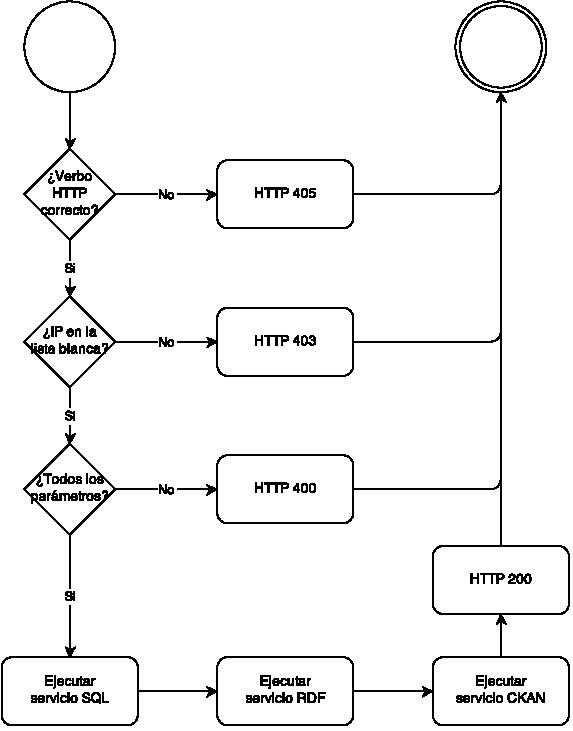
\includegraphics[width=\textwidth]{actividad/actividad_receiver}
	\caption{Diagrama de actividad del proceso de importación de datos}
	\label{fig:diagrama_actividad_receiver}
\end{figure}



\subsection{Funcionamiento del framework de soporte a visualizaciones}
\label{actividad:framework_visualizaciones}
A continuación se explicará el funcionamiento del framework que provee los datos necesarios para crear las visualizaciones.  Anteriormente, en la ``\nameref{vista_sistema}'' se explicó que éste componente se sitúa dentro del CMS y forma parte del subsistema de datos y se encarga de ofrecer los datos que se utilizarán por las visualizaciones para presentarlos de forma gráfica al usuario.  La arquitectura de éste componente pude verse en detalle en la  ``\nameref{vista_landportal_uris}'' del presente capítulo.

La figura \ref{fig:diagrama_actividad_framework_soporte_visualizaciones} muestra el diagrama de actividad de éste componente.  Los siguientes pasos tienen lugar durante su actividad.
\begin{enumerate}
	\item  En primer lugar, el framework recibe una petición de datos por parte de una visualización para mostrarlos de forma gráfica a un usuario.
	\item  El primer paso que tiene lugar es la extracción de parámetros de la petición.  Por ejemplo: en caso de necesitar datos sobre una determinada región, uno de los parámetros será el identificador de dicha región.
	\item  El segundo paso consiste en comprobar si el sistema ha recibido alguna petición similar anteriormente y, por tanto se encuentra almacenada en el caché.  En caso de que una petición anterior con los mismos parámetros se encontrara cacheada, el sistema devuelve los datos del caché y finaliza la ejecución.
	\item  Si no hay cacheada ninguna petición similar anterior será necesario extraer los datos de la base de datos y construir una respuesta.
		\begin{enumerate}
			\item  Primeramente se abre una nueva conexión con la base de datos.  La conexión se realiza a través del componente \textit{DatabaseHelper}, como se puede comprobar en la ``\nameref{vista_landportal_uris}''.
			\item  Posteriormente se procede al escapado de los argumentos que llegaron originalmente en la petición.  Éste proceso es necesario para evitar posibles ataques del tipo \textit{SQL Injection}\footnote{Una inyección de código SQL o \textit{SQL Injection} es un mecanismo de ataque que permite alterar las consultas SQL para obtener información oculta, modificar la información almacenada en la base de datos o ejecutar instrucciones del sistema de gestión de base de datos.  Para obtener más información sobre se recomienda ver la entrada del manual de PHP a cerca de éste tema en \url{http://php.net/manual/en/security.database.sql-injection.php}}.
			\item  Tras garantizar que los parámetros recibidos son seguros, el sistema procede a realizar las consultas necesarias a la base de datos y recibir la información que devolverá posteriormente.
			\item  Una vez se haya terminado de trabajar con la base de datos, se cerrará la conexión puesto que no se volverá a utilizar posteriormente.
		\end{enumerate}
	\item  Cuando ya se han obtenido todos los datos necesarios de la base de datos y se haya cerrado la conexión, el sistema procesará los datos para transformarlos al formato JSON en el que se enviará la respuesta.
	\item  Una vez que los datos ya se encuentran en formato JSON y listos para ser devueltos, el sistema los almacenará en el caché para que, como ya se ha explicado anteriormente, las posteriores peticiones similares no tengan que volver a consultar la base de datos ni volver a procesar los resultados.
	\item  Por último, se devolverán los datos ya procesados en formato JSON para que sean utilizados por las visualizaciones.
\end{enumerate}
\begin{figure}[h]
	\centering
	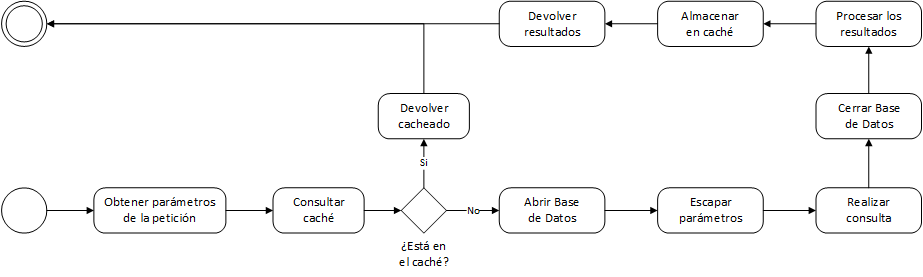
\includegraphics[width=\textwidth]{actividad/actividad_framework_visualizaciones}
	\caption{Diagrama de actividad del framework de soporte a visualizaciones}
	\label{fig:diagrama_actividad_framework_soporte_visualizaciones}
\end{figure}

El anexo \ref{anexo_vista_personalizada} contiene una guía que explica en detalle el proceso de creación de plantillas personalizadas.

\subsection{Llamada a las plantillas de la sección de datos}
\label{actividad:landportal-uris_theme}
A continuación se explicará el funcionamiento del módulo ``\textit{landportal-uris}'' en conjunción con el tema del CMS.  En la ``\nameref{vista_modulos_cms}'' puede verse con detalle la organización de ambos componentes como parte del gestor de contenidos.

La figura \ref{fig:diagrama_actividad_vistas} muestra el diagrama de actividad de las llamadas a las plantillas del tema por parte del módulo ``\textit{landportal-uris}''.  Cabe destacar que éste diagrama sólo es aplicable a las plantillas pertenecientes a la sección de datos, puesto que las plantillas de la sección social serán llamadas directamente por el núcleo de Drupal\footnote{El mecanismo utilizado por el núcleo de Drupal para seleccionar las plantillas recibe el nombre de ``\textit{template suggestions}''.  Para más información se recomienda ver el contenido de la documentación de Drupal al respecto en \url{https://www.drupal.org/node/1089656}}.  La actividad está formada por los siguientes pasos:
\begin{enumerate}
	\item  En primer lugar, cuando el módulo recibe una petición invoca a un \textit{callback} que se encarga de seleccionar tanto el modelo como la plantilla adecuados.
		\begin{enumerate}
			\item  Como se verá posteriormente, el modelo es el encargado de obtener los datos con los que se rellenarán las vistas.  El modelo adecuado para una petición se obtiene mediante un convenio de nombres, por ejemplo una petición a la ruta \textit{country} instanciará el modelo \textit{Country}, de éste modo la creación de nuevas rutas no requiere ningún tipo de configuración adicional.
			\item  La plantilla contiene el código HTML que se mostrará al usuario.  La plantilla adecuada se obtiene utilizando un convenio de nombres de forma similar a como sucede con el modelo.
		\end{enumerate}
	\item  Una vez que se ha obtenido el modelo se procederá a pedirle sus datos.  En este punto es necesario mencionar que la forma en la que los modelos obtienen sus datos es similar a la forma en la que lo hacen las clases del framework de soporte a las visualizaciones.  Todo lo explicado en la sección anterior (``\nameref{actividad:framework_visualizaciones})'' es también aplicable aquí.
	\item  En caso de que el modelo no devolviera ningún dato indicaría que los parámetros de la petición son incorrectos y, por tanto, la plantilla se cambiará para mostrar un error 404.
	\item  Tanto si el modelo ha obtenido datos o no, se realizará un preprocesado de la plantilla.  El preprocesado permite incluir algunas variables comunes que son utilizadas por todas las plantillas.
	\item  Por último se renderizará la plantilla para incluir todos los datos obtenidos del modelo y se devolverá el código HTML resultante al usuario que realizó la petición.
\end{enumerate}

\begin{figure}[h]
	\centering
	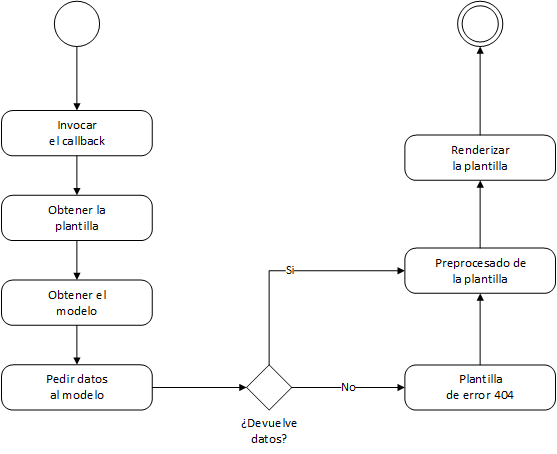
\includegraphics[width=\textwidth]{actividad/actividad_modulo_vistas}
	\caption{Diagrama de actividad de la llamada a las plantillas en la sección de datos}
	\label{fig:diagrama_actividad_vistas}
\end{figure}